% Options for packages loaded elsewhere
\PassOptionsToPackage{unicode}{hyperref}
\PassOptionsToPackage{hyphens}{url}
%
\documentclass[
]{article}
\usepackage{amsmath,amssymb}
\usepackage{lmodern}
\usepackage{ifxetex,ifluatex}
\ifnum 0\ifxetex 1\fi\ifluatex 1\fi=0 % if pdftex
  \usepackage[T1]{fontenc}
  \usepackage[utf8]{inputenc}
  \usepackage{textcomp} % provide euro and other symbols
\else % if luatex or xetex
  \usepackage{unicode-math}
  \defaultfontfeatures{Scale=MatchLowercase}
  \defaultfontfeatures[\rmfamily]{Ligatures=TeX,Scale=1}
\fi
% Use upquote if available, for straight quotes in verbatim environments
\IfFileExists{upquote.sty}{\usepackage{upquote}}{}
\IfFileExists{microtype.sty}{% use microtype if available
  \usepackage[]{microtype}
  \UseMicrotypeSet[protrusion]{basicmath} % disable protrusion for tt fonts
}{}
\makeatletter
\@ifundefined{KOMAClassName}{% if non-KOMA class
  \IfFileExists{parskip.sty}{%
    \usepackage{parskip}
  }{% else
    \setlength{\parindent}{0pt}
    \setlength{\parskip}{6pt plus 2pt minus 1pt}}
}{% if KOMA class
  \KOMAoptions{parskip=half}}
\makeatother
\usepackage{xcolor}
\IfFileExists{xurl.sty}{\usepackage{xurl}}{} % add URL line breaks if available
\IfFileExists{bookmark.sty}{\usepackage{bookmark}}{\usepackage{hyperref}}
\hypersetup{
  pdftitle={Forecasting CO2 emissions using ARIMA models in Brazil, China, EU, India and US},
  pdfauthor={Daniel Bustillo Mac Lean},
  hidelinks,
  pdfcreator={LaTeX via pandoc}}
\urlstyle{same} % disable monospaced font for URLs
\usepackage[margin=1in]{geometry}
\usepackage{graphicx}
\makeatletter
\def\maxwidth{\ifdim\Gin@nat@width>\linewidth\linewidth\else\Gin@nat@width\fi}
\def\maxheight{\ifdim\Gin@nat@height>\textheight\textheight\else\Gin@nat@height\fi}
\makeatother
% Scale images if necessary, so that they will not overflow the page
% margins by default, and it is still possible to overwrite the defaults
% using explicit options in \includegraphics[width, height, ...]{}
\setkeys{Gin}{width=\maxwidth,height=\maxheight,keepaspectratio}
% Set default figure placement to htbp
\makeatletter
\def\fps@figure{htbp}
\makeatother
\setlength{\emergencystretch}{3em} % prevent overfull lines
\providecommand{\tightlist}{%
  \setlength{\itemsep}{0pt}\setlength{\parskip}{0pt}}
\setcounter{secnumdepth}{-\maxdimen} % remove section numbering
\usepackage{booktabs}
\usepackage{longtable}
\usepackage{array}
\usepackage{multirow}
\usepackage{wrapfig}
\usepackage{float}
\usepackage{colortbl}
\usepackage{pdflscape}
\usepackage{tabu}
\usepackage{threeparttable}
\usepackage{threeparttablex}
\usepackage[normalem]{ulem}
\usepackage{makecell}
\usepackage{xcolor}
\ifluatex
  \usepackage{selnolig}  % disable illegal ligatures
\fi
\usepackage[]{natbib}
\bibliographystyle{plainnat}

\title{Forecasting CO2 emissions using ARIMA models in Brazil, China,
EU, India and US}
\usepackage{etoolbox}
\makeatletter
\providecommand{\subtitle}[1]{% add subtitle to \maketitle
  \apptocmd{\@title}{\par {\large #1 \par}}{}{}
}
\makeatother
\subtitle{Time Series Analysis Term Paper}
\author{Daniel Bustillo Mac Lean}
\date{31-08-2021}

\begin{document}
\maketitle

{
\setcounter{tocdepth}{2}
\tableofcontents
}
\hypertarget{motivation}{%
\section{Motivation}\label{motivation}}

Increasing evidence has shown that human emissions of carbon dioxide and
other greenhouse gases are a primary driver of climate change
(\citet{stocker2014climate}). This makes worldwide emissions one of the
world's most pressing challenges and has provoked various international
agreement, like the Paris Agreement on emission reduction and other
climate goals. Three of the largest current emitting regions are China,
the US and the EU.

\newpage

\hypertarget{introduction}{%
\section{Introduction}\label{introduction}}

The main topic of this term paper is to analyze and model the trends of
CO2 emissions in some of the countries of the European Union, the United
States of America and China (and perhaps comparing them with emerging
economics such as Brazil and India). Current actions to mitigate the
climate effects of such steep rise of CO2 emissions over the last 50-60
years are not enough to reach the goals set in the Paris Agreement by
2030. Such is the slow response from the governing institutions and
international organizations that the current trends indicate that the
temperature increases (and all the consequences behind it) will be
irreversible in the future. This paper will analyze the trends of CO2
emissions of the above-mentioned countries and will design a fitting
Auto Regressive Integrated Moving Average (ARIMA) model. Next, we will
run diagnostics and perform the necessary tests to assure that the model
accounts for stationarity and possibly seasonality. Lastly, a forecast
for the next periods based on the model will be presented.

\hypertarget{literature-review}{%
\section{Literature review}\label{literature-review}}

There have been several studies that apply ARIMA models and similar
statistical and econometric techniques to forecast carbon dioxide
emissions for different regions, countries and time periods.

\citet{fatima2019forecasting} used Simple Exponential Smoothing (SES)
and ARIMA models to forecast CO2 emissions for several Asian countries,
with China and India among them. For China they fit an (1,2,0) ARIMA
model and for India an (0,2,1) ARIMA model.

\citet{nyoni2019modeling} modeled an ARIMA model for CO2 emissions in
China for the period 1960-2014, they found that an ARIMA(1,2,1) model is
the most suitable model to forecast total annual CO2 emissions for
China.

A study on carbon dioxide emissions between 1972 and 2015 in Bangladesh
was conducted by \citet{rahman2017modeling}. According to their results,
the best fitting ARIMA model was of order (0,2,1).

One of the justifications some of these authors mention when choosing to
forecast using ARIMA models was that no other data is necessary, the
forecasting can be done using only historical values of the data, with
no other variables involved.

\hypertarget{the-model-and-data}{%
\section{The model and data}\label{the-model-and-data}}

In this section, we go over the data, its characteristics, sources and
reliability. Moreover, we introduce the ARIMA (Auto Regressive
Integrated Moving Average) model in a formal way, next, we run the model
on our data to then set up all the insights to analyze in the following
section.

All data is taken from the World Bank's Database. This database has
proven to be reliable for industrialized countries, not so much for
developing countries, since data from these countries might not be
recollected or administered correctly by the corresponding authorities.

As stated in the Introduction, our interest here is to analyze the
trends of the 3 biggest emitters of CO2 in the world: the United States
of America, the European Union and China . Additionally, we compare
those trends and forecast, with trends and forecast of emerging
economies such as Brazil and India, as those countries display worrying
trends on CO2 emissions that are product of contamination and
deforestation due to their growing industries.

The measure we use for our analysis is C02 emissions per capita, because
although all country groups are the among the biggest in terms of
surface, the population density is different and thus ``spreading'' the
CO2 emissions by population gives us more sensible data and accounted
for the different sizes of population.

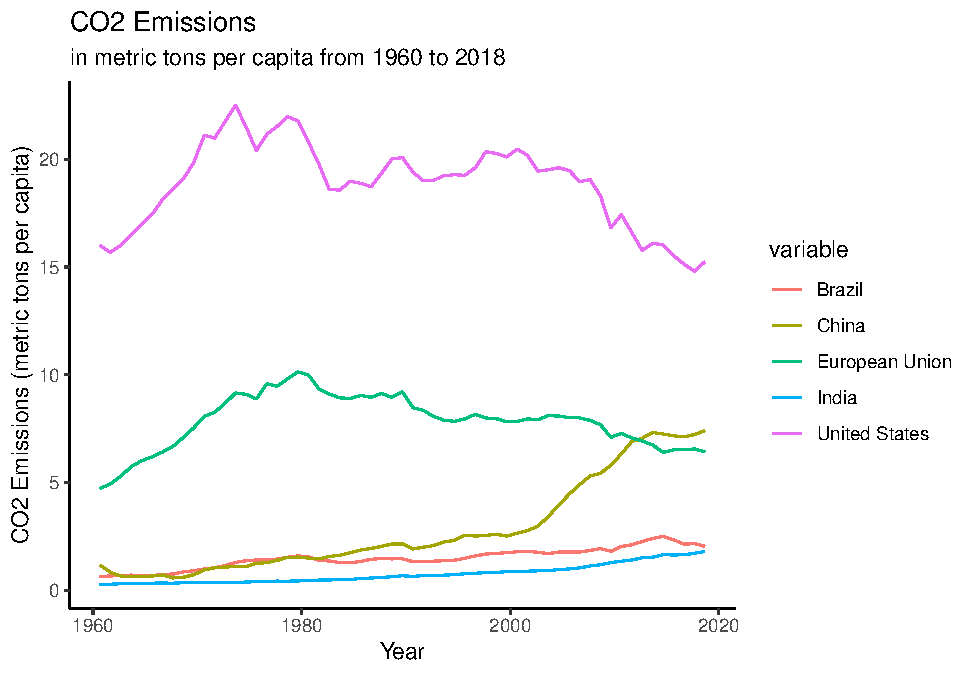
\includegraphics{tsa_files/figure-latex/unnamed-chunk-1-1.pdf}

As seen above, CO2 emissions of the countries of interest are showing
different trends and magnitudes.\footnote{For a more detailed view of
  each countries' time series see next section of the paper}

Even though the European Union and the United States show some decline
in emissions after the 1980s, the level of emissions are significantly
higher than emerging countries like Brazil or India. The worrying part
is that China's carbon dioxide emissions surpassed the ones from the
European Union in the last 10 years, the steep rise since the early
2000s matches Chinas rising role as a main actor in the global economy.

Below are the summary statistics for all countries and their respective
time series plots (the time period of the data recollected is from 1960
to 2018 for all countries)

\begin{table}

\caption{\label{tab:sumstats}Summary statistics for all countries}
\centering
\begin{tabular}[t]{l|l|l|l|l|l}
\hline
  &     Brazil &     China & European Union &     India & United States\\
\hline
 & Min.   :0.6499 & Min.   :0.5742 & Min.   : 4.729 & Min.   :0.2676 & Min.   :14.81\\
\hline
 & 1st Qu.:1.2913 & 1st Qu.:1.2103 & 1st Qu.: 7.000 & 1st Qu.:0.3929 & 1st Qu.:17.44\\
\hline
 & Median :1.4577 & Median :2.0384 & Median : 7.966 & Median :0.6441 & Median :19.24\\
\hline
 & Mean   :1.4862 & Mean   :2.8182 & Mean   : 7.845 & Mean   :0.7551 & Mean   :18.86\\
\hline
 & 3rd Qu.:1.7758 & 3rd Qu.:3.6886 & 3rd Qu.: 8.914 & 3rd Qu.:0.9382 & 3rd Qu.:20.14\\
\hline
 & Max.   :2.4994 & Max.   :7.4052 & Max.   :10.133 & Max.   :1.7998 & Max.   :22.51\\
\hline
\end{tabular}
\end{table}

\newpage

\hypertarget{individual-time-series-plots}{%
\subsubsection{Individual Time series
plots}\label{individual-time-series-plots}}

To have a more detailed view of each countries dioxide emissions we plot
each time series plot individually.

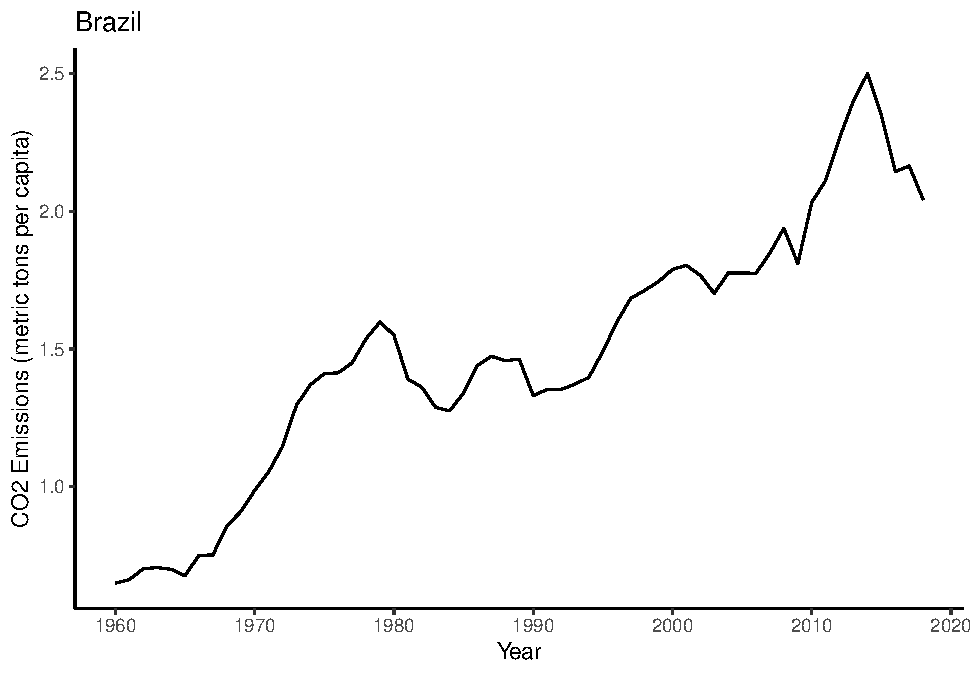
\includegraphics[width=0.5\linewidth]{tsa_files/figure-latex/descrstats-1}
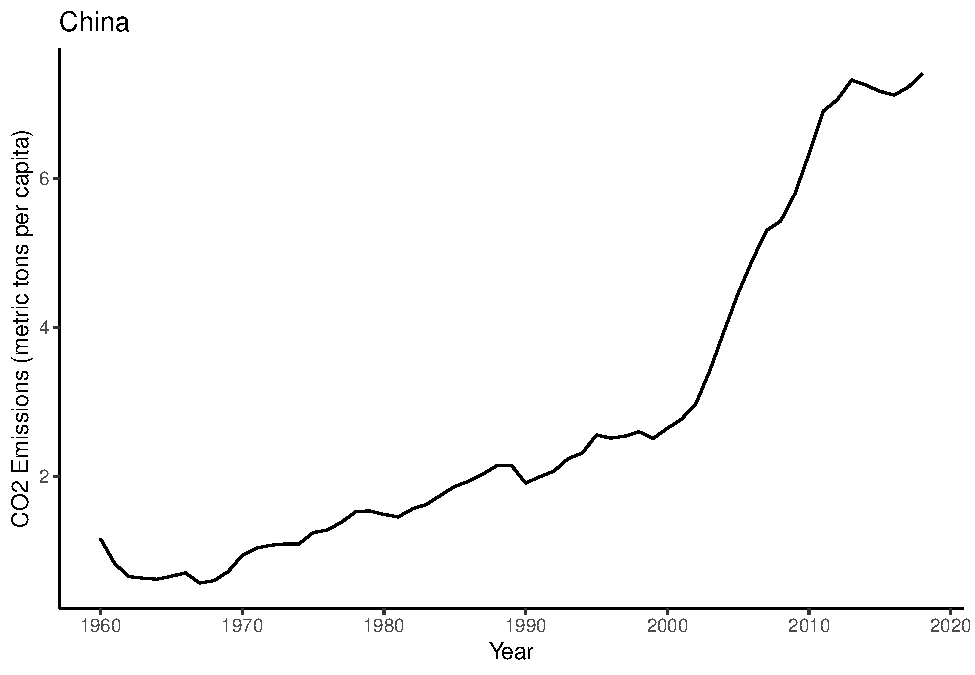
\includegraphics[width=0.5\linewidth]{tsa_files/figure-latex/descrstats-2}
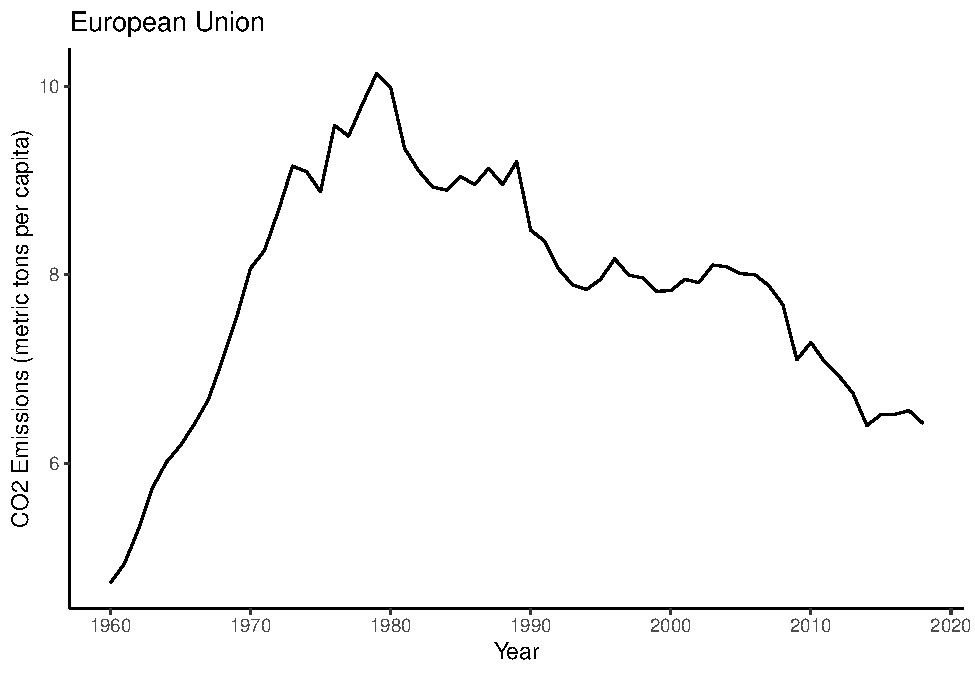
\includegraphics[width=0.5\linewidth]{tsa_files/figure-latex/descrstats-3}
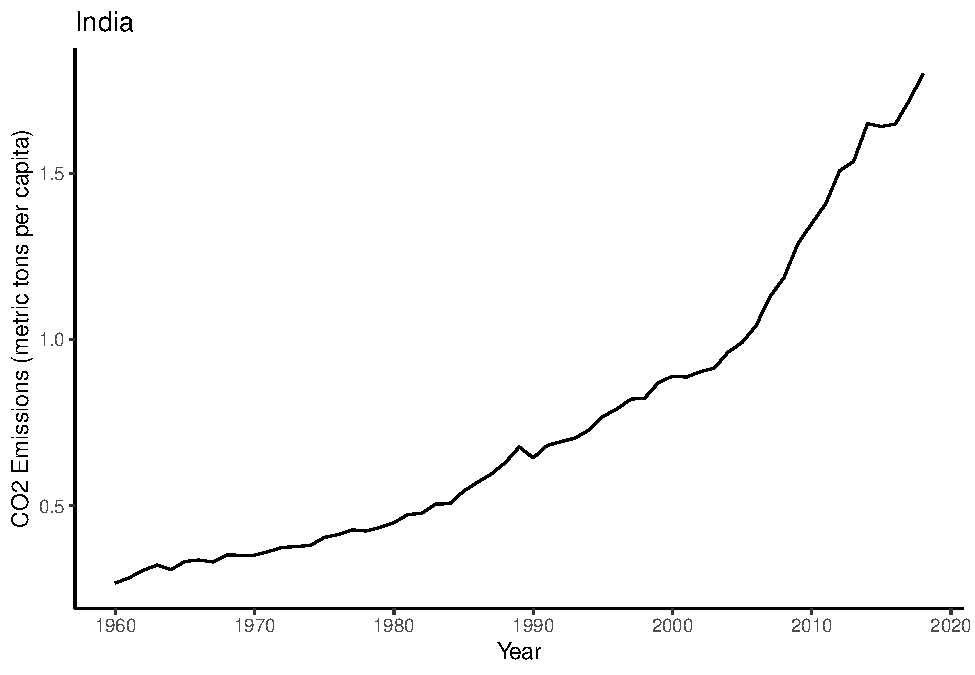
\includegraphics[width=0.5\linewidth]{tsa_files/figure-latex/descrstats-4}
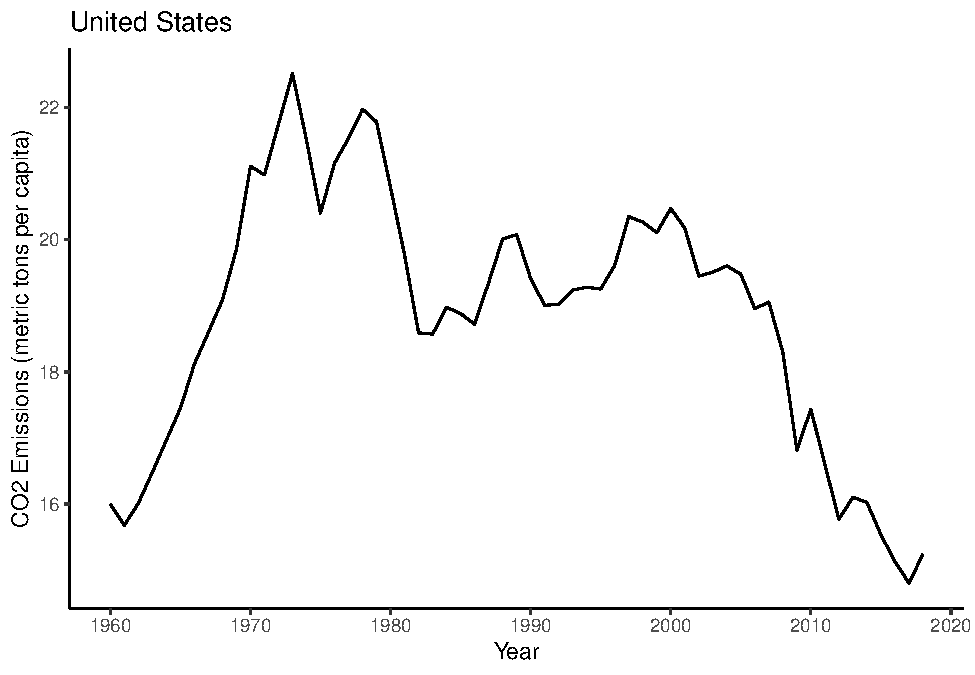
\includegraphics[width=0.5\linewidth]{tsa_files/figure-latex/descrstats-5}

Plotting the time series individually makes it evident that all series
aren't stationary, as they show different trends. In the case of Brazil,
China and India, their emissions have been rising over the last 50 years
and there is positive trend. In the EU and the US, the case is
different, but they appear to be non-stationary.

\newpage

\hypertarget{autocorrelation-plots-and-partial-autocorrelation-plots}{%
\subsubsection{Autocorrelation plots and Partial Autocorrelation
plots}\label{autocorrelation-plots-and-partial-autocorrelation-plots}}

Using the autocorrelation function formula: \[\rho_k =
\frac{\gamma_k}{\gamma_o}=\frac{Cov[y_t,y_{t-k}]}{Var(y_t)}\] all ACF
are calculated for each country group. This works as a visual way to
determine if a time series object is stationary or not. In the next
section we run the necessary test to confirm our findings from the ACFS.

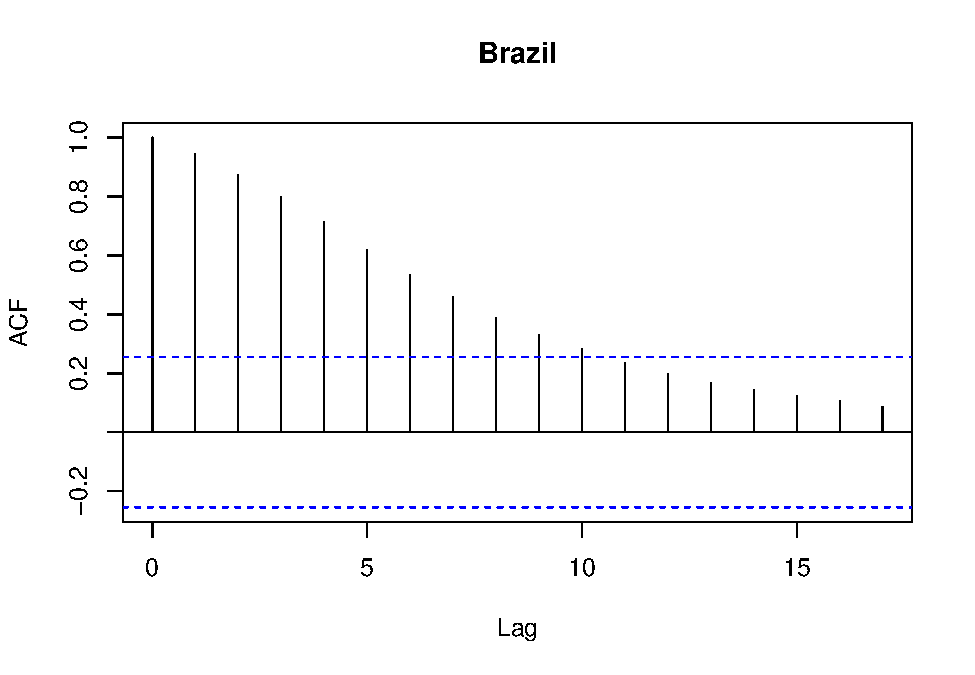
\includegraphics[width=0.5\linewidth]{tsa_files/figure-latex/acfs_plots-1}
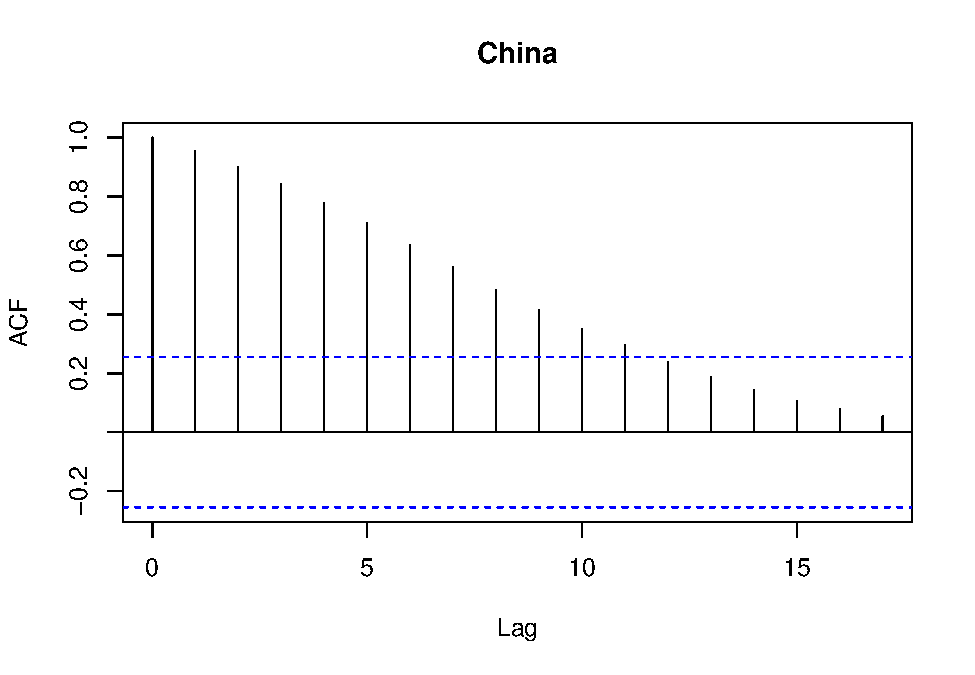
\includegraphics[width=0.5\linewidth]{tsa_files/figure-latex/acfs_plots-2}
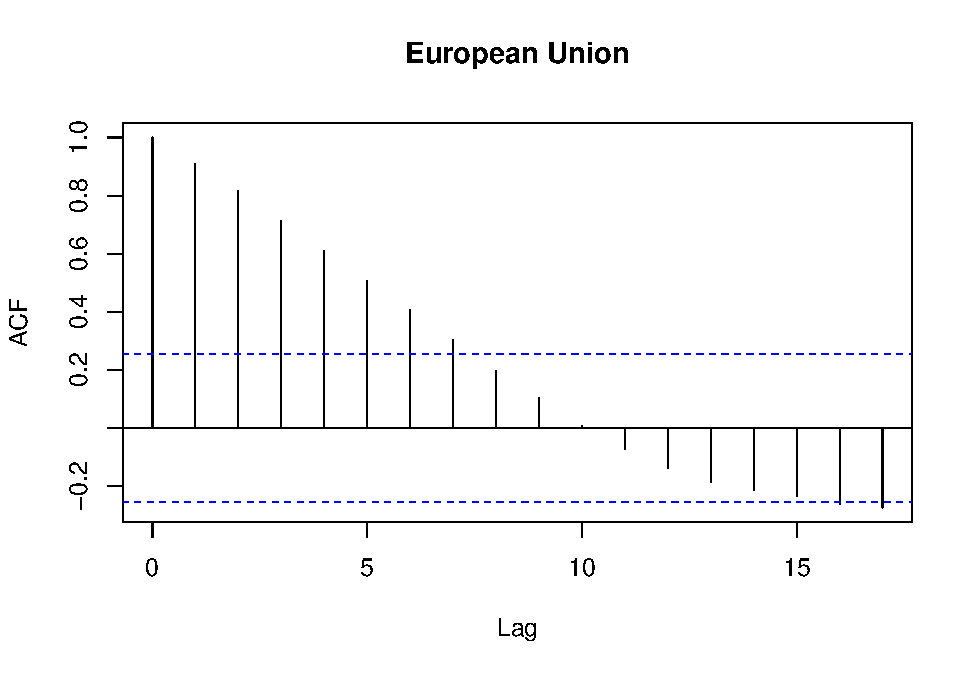
\includegraphics[width=0.5\linewidth]{tsa_files/figure-latex/acfs_plots-3}
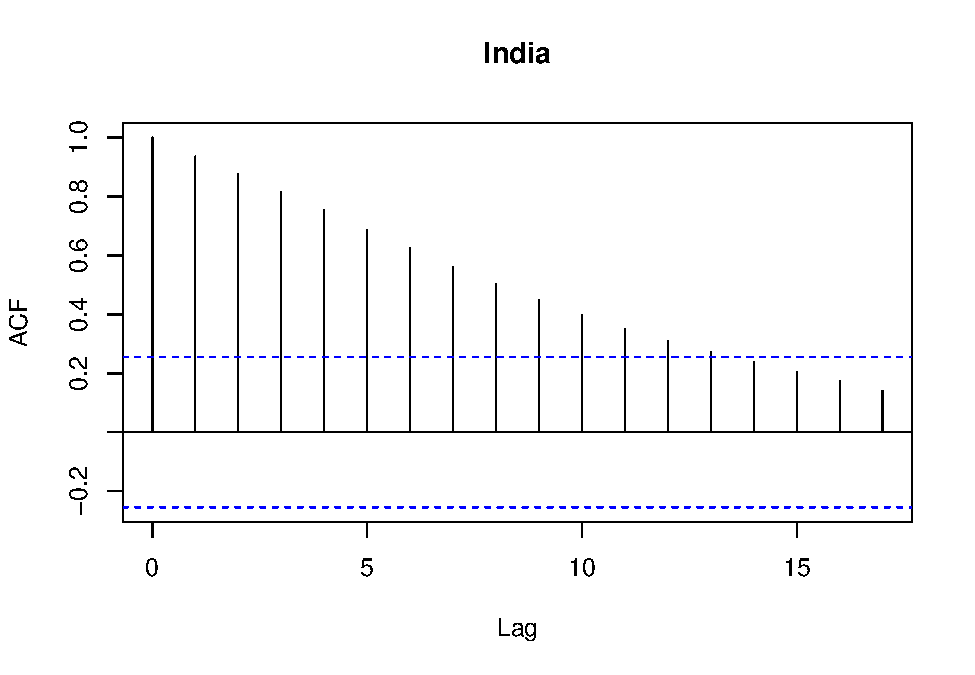
\includegraphics[width=0.5\linewidth]{tsa_files/figure-latex/acfs_plots-4}
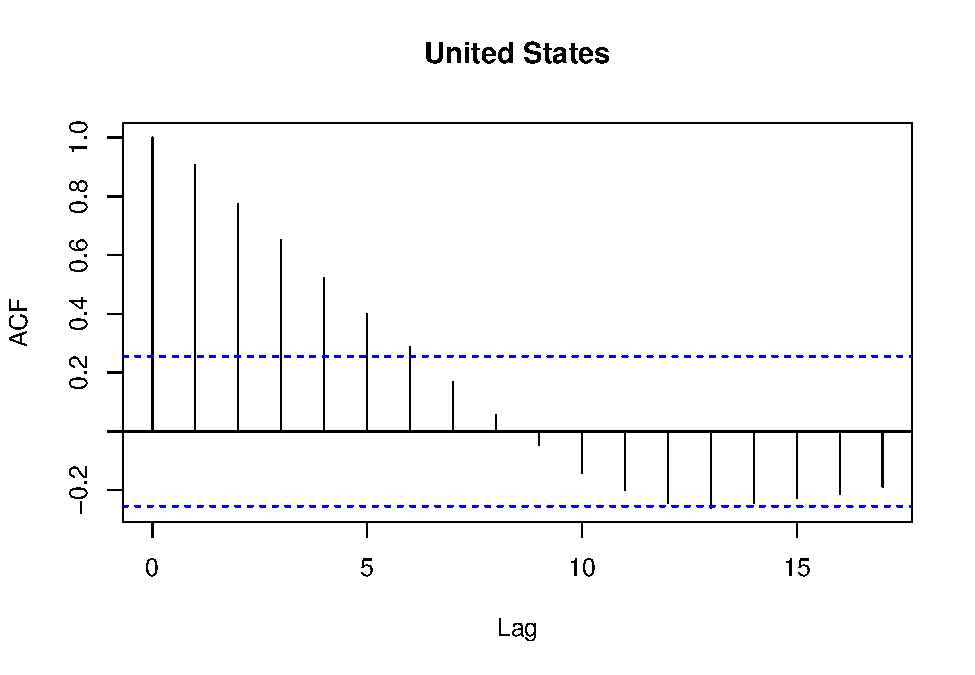
\includegraphics[width=0.5\linewidth]{tsa_files/figure-latex/acfs_plots-5}

To further assist with our model choice, we use the Partial
Autocorrelation Functions plots as well.

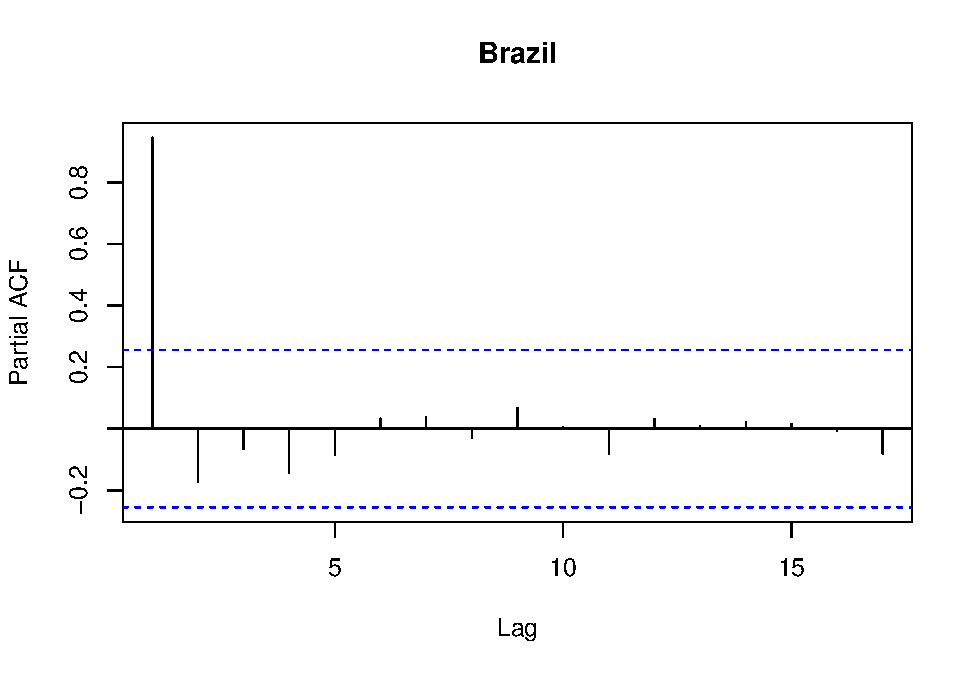
\includegraphics[width=0.5\linewidth]{tsa_files/figure-latex/pacf-1}
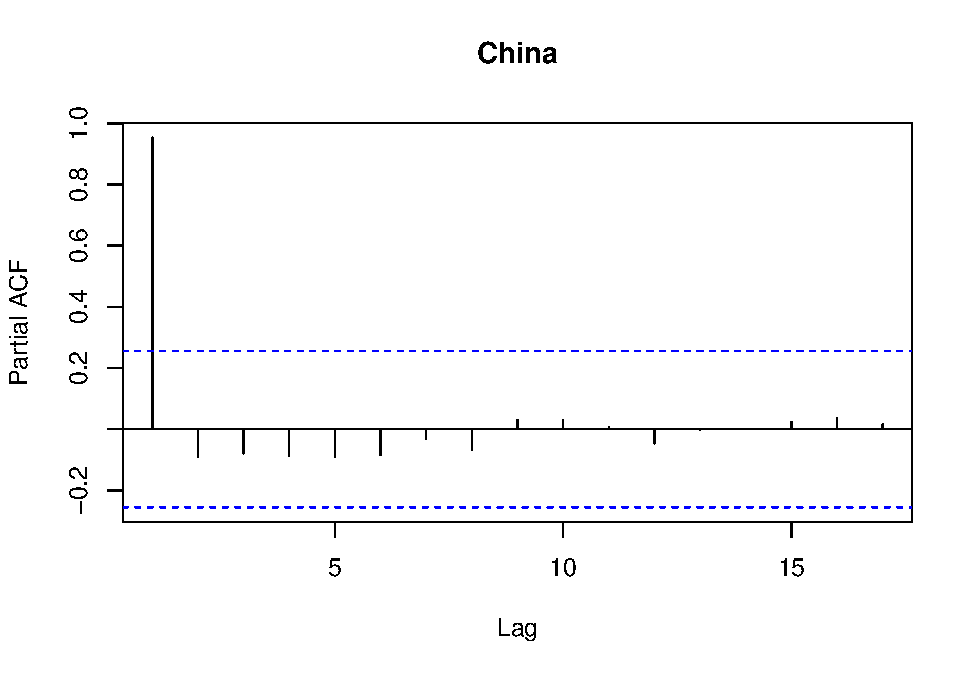
\includegraphics[width=0.5\linewidth]{tsa_files/figure-latex/pacf-2}
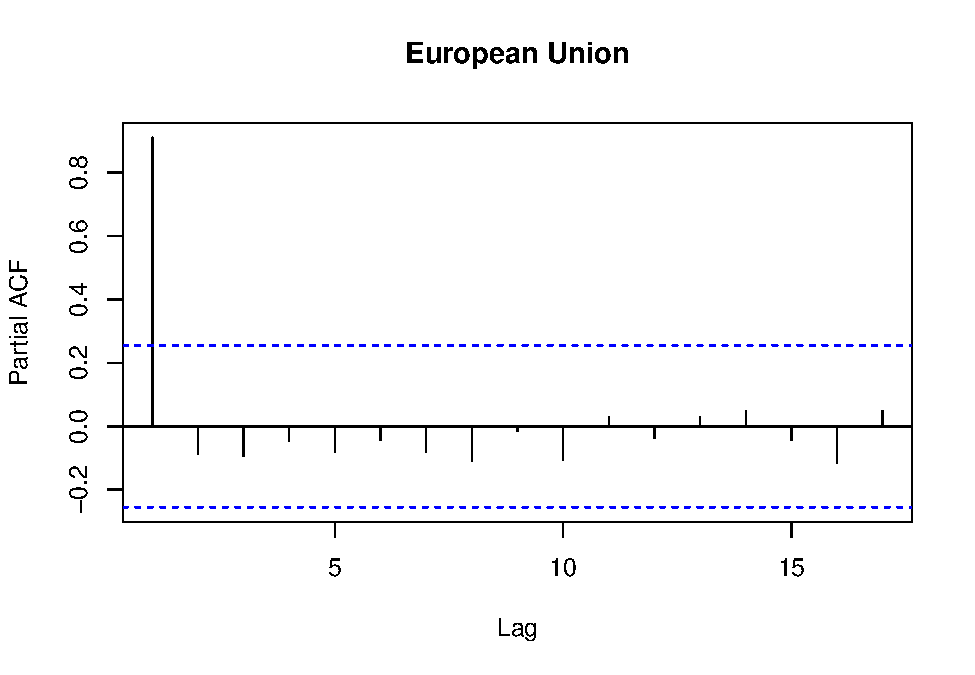
\includegraphics[width=0.5\linewidth]{tsa_files/figure-latex/pacf-3}
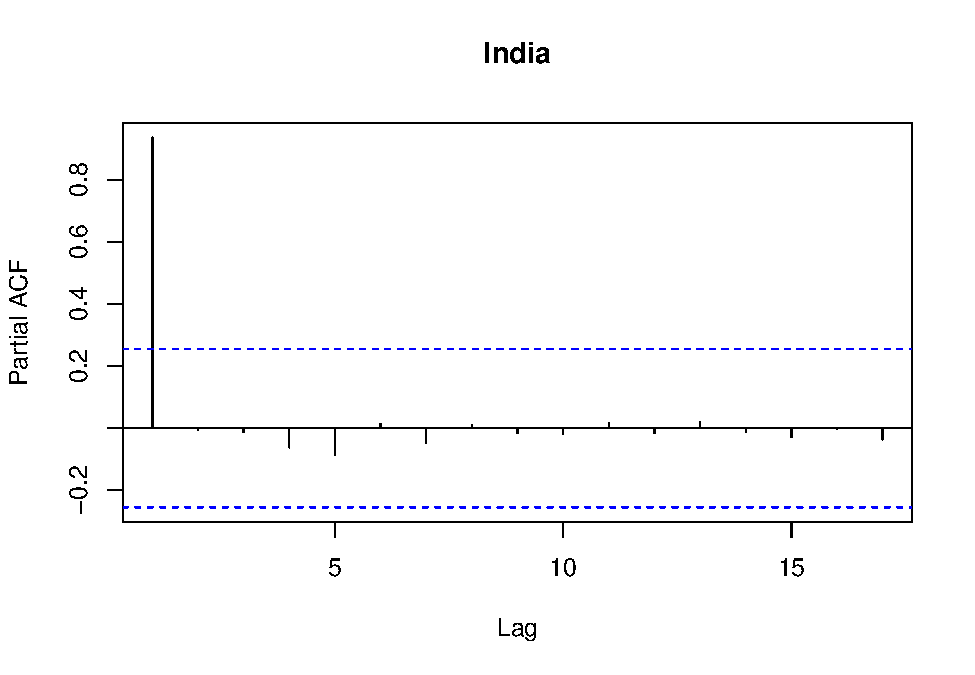
\includegraphics[width=0.5\linewidth]{tsa_files/figure-latex/pacf-4}
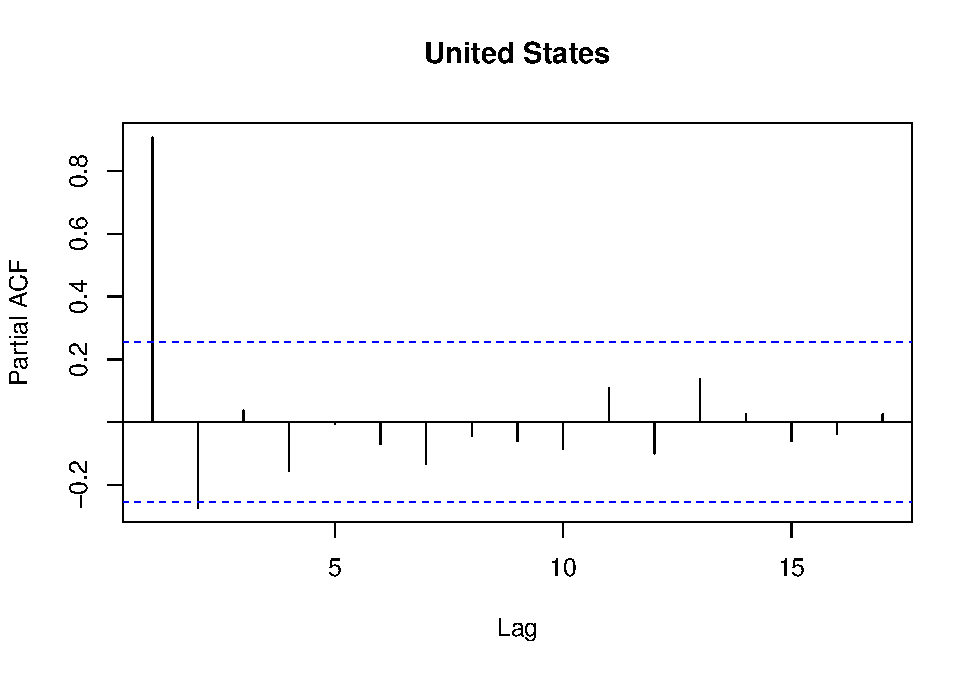
\includegraphics[width=0.5\linewidth]{tsa_files/figure-latex/pacf-5}

\newpage

\hypertarget{stationarity-tests}{%
\section{Stationarity tests}\label{stationarity-tests}}

\hypertarget{augmented-dickey-fuller-test}{%
\subsubsection{Augmented Dickey Fuller
Test}\label{augmented-dickey-fuller-test}}

With this test we want to negate the null hypothesis that a unit root is
present in an auto regressive model of a given time series, and that the
process is thus not stationary.

A common rule of thumb for determining pmax, suggested by
\citet{schwert1989business}, is \[ p_{max}=[12(\frac{T}{100})^{1/4}]\]

\hypertarget{kpss-unit-root-test}{%
\subsubsection{KPSS Unit Root Test}\label{kpss-unit-root-test}}

We also use the KPSS Unit Root test from \citet{kwiatkowski1992testing}
to test the H0 hypothesis of stationarity.

\begin{table}[H]

\caption{\label{tab:tabunit}p-values for ADF and KPSS Tests}
\centering
\begin{tabular}[t]{l|r|r}
\hline
  &  ADF p-value & KPSS p-value\\
\hline
Brazil & 0.0359389 & 0.0208252\\
\hline
China & 0.4486139 & 0.0248861\\
\hline
European Union & 0.0064731 & 0.1000000\\
\hline
India & 0.9751775 & 0.0209267\\
\hline
United States & 0.1702564 & 0.1000000\\
\hline
\end{tabular}
\end{table}

Based on the table above , results from the Augmented Dickey Fuller Test
and the KPSS Test, we can only reject the ADF H0 hypothesis of
non-stationarity for Brazil and the European Union. On the contrary,
KPSS p-values show that we might reject the H0 hypothesis of
stationarity for Brazil, China and India.

\newpage

\hypertarget{estimation-and-results}{%
\section{Estimation and results}\label{estimation-and-results}}

Having conducted the necessary test and evaluated al the different time
series and their characteristics, it is time to estimate a model,
present, analyze and interpret the results.

For the estimation of the ARIMA model we ran a so-called
\href{https://www.r-bloggers.com/2018/11/searching-for-the-optimal-hyper-parameters-of-an-arima-model-in-parallel-the-tidy-gridsearch-approach/}{Grid-Search}
for the 5 different country groups and all possible combinations of
models within our parameters. We then evaluate the best model for each
country based on the Akaike Information Criterion :
\[ AIC=log(\hat{\sigma}^2_{\epsilon}) + 2\frac{p+q+1}{T}\] Having
defined the maximal \emph{p} order in the previous section (11 lags), we
restricted the \emph{d} order to 3, as too many differentiation of the
time series don't bring better results. Moreover, we restrict the
\emph{q} parameter from the MA(q) model to 11.

Below there is a table with each countries' best models and their
respective AIC coefficients.

\begin{table}[H]
\centering
\begin{tabular}{l|l|l}
\hline
Country & Order & AIC\\
\hline
Brazil & (2,1,5) & -127.6029\\
\hline
China & (1,1,0) & -61.7693\\
\hline
European Union & (0,2,1) & 10.93498\\
\hline
India & (1,1,2) & -254.3758\\
\hline
United States & (0,1,1) & 98.9266\\
\hline
\end{tabular}
\end{table}

We compared the results with results from the \textbf{auto.arima}
function from the \emph{forecast} package, and they match for all the
countries, although the \textbf{auto.arima} function required some extra
tweaking. In the end, we choose the models that display the lowest AIC
values.

\hypertarget{diagnostics}{%
\subsubsection{Diagnostics}\label{diagnostics}}

Next we proceed to run diagnostics of our models, that means that our
model should capture the dynamics of the time series. Consequently, the
residuals should be approximately white noise (No residual correlation,
same variance, normally distributed). We do this with the Ljung-Box
Test:
\[ Q_K= T( T+2) \sum^K_{k=1}\frac{1}{T-k}\hat{\rho}^2_k  \longrightarrow \chi^2 (K -p-q)  \]

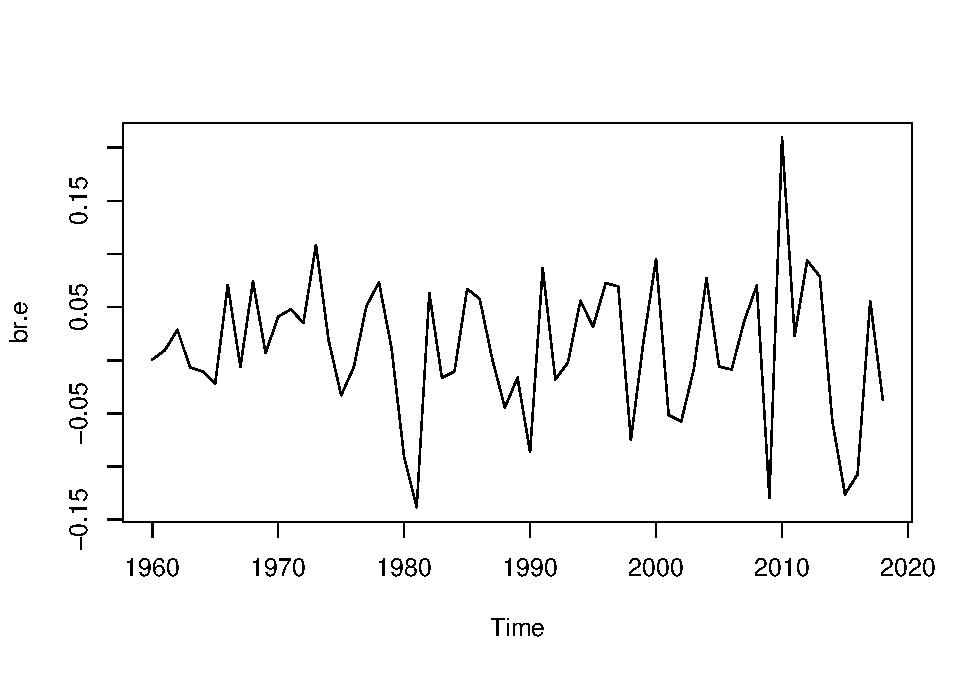
\includegraphics[width=0.5\linewidth]{tsa_files/figure-latex/resid-1}
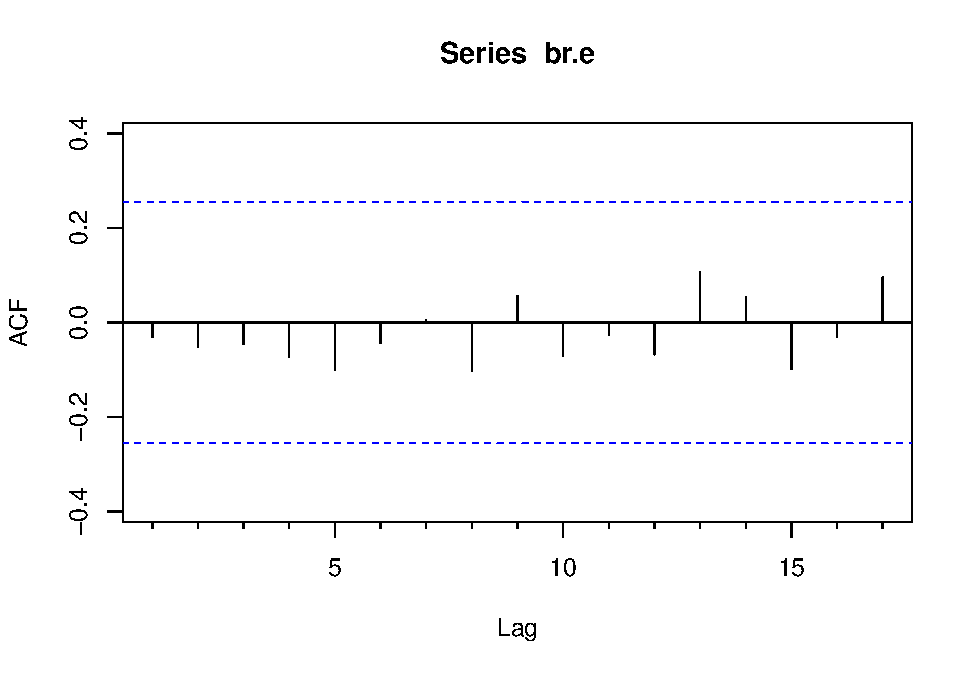
\includegraphics[width=0.5\linewidth]{tsa_files/figure-latex/resid-2}
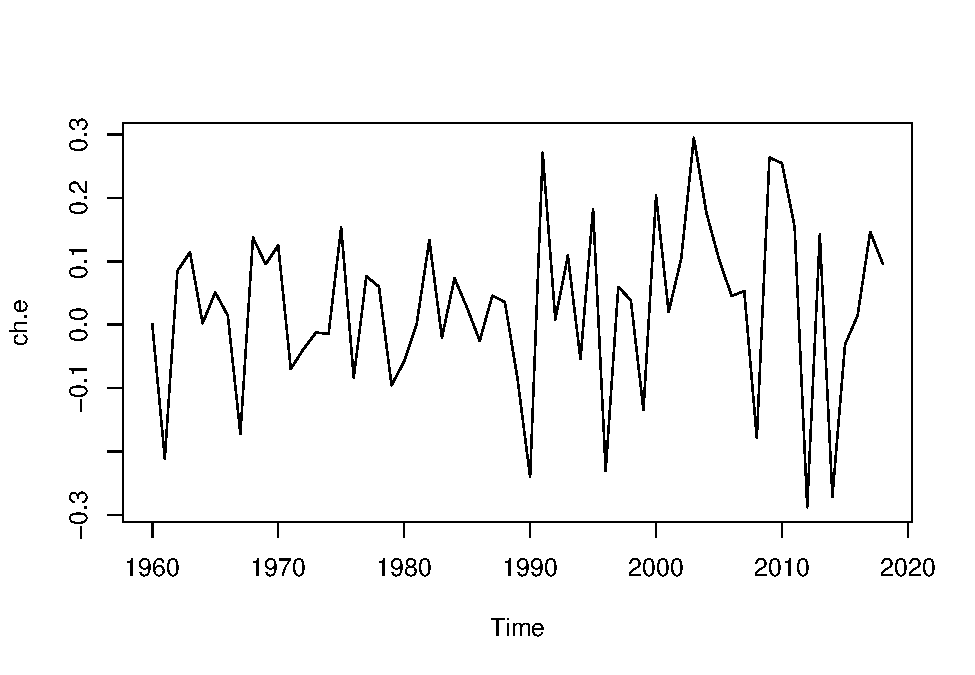
\includegraphics[width=0.5\linewidth]{tsa_files/figure-latex/resid-3}
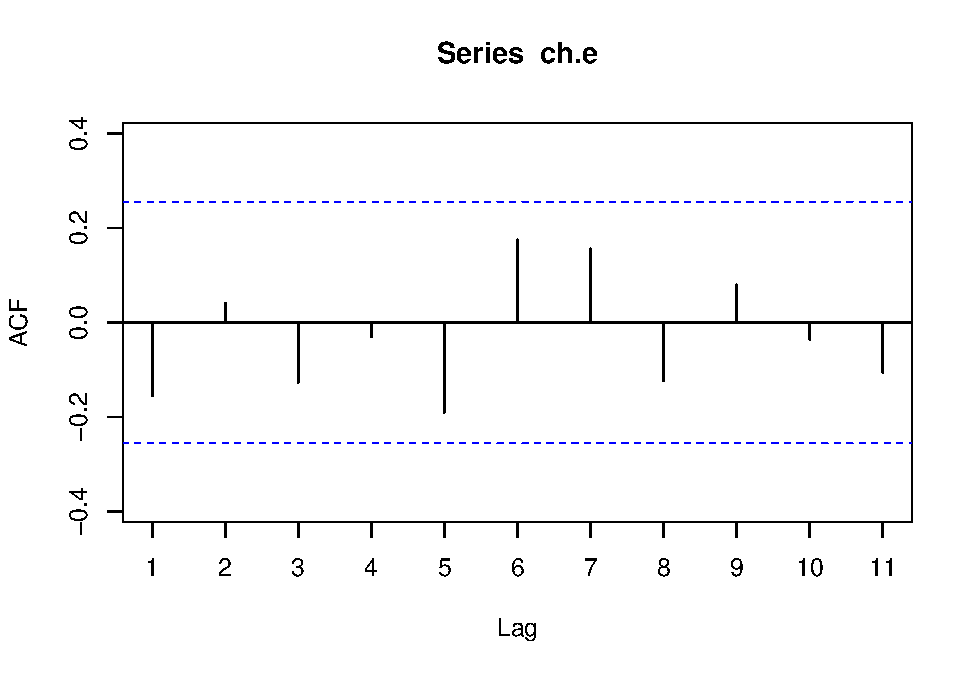
\includegraphics[width=0.5\linewidth]{tsa_files/figure-latex/resid-4}
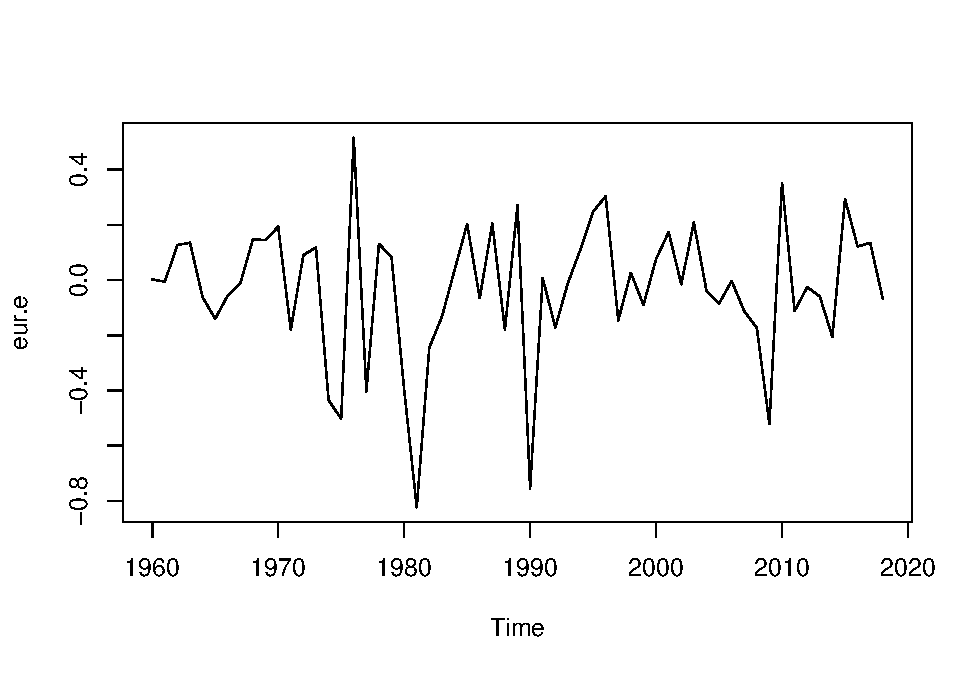
\includegraphics[width=0.5\linewidth]{tsa_files/figure-latex/resid-5}
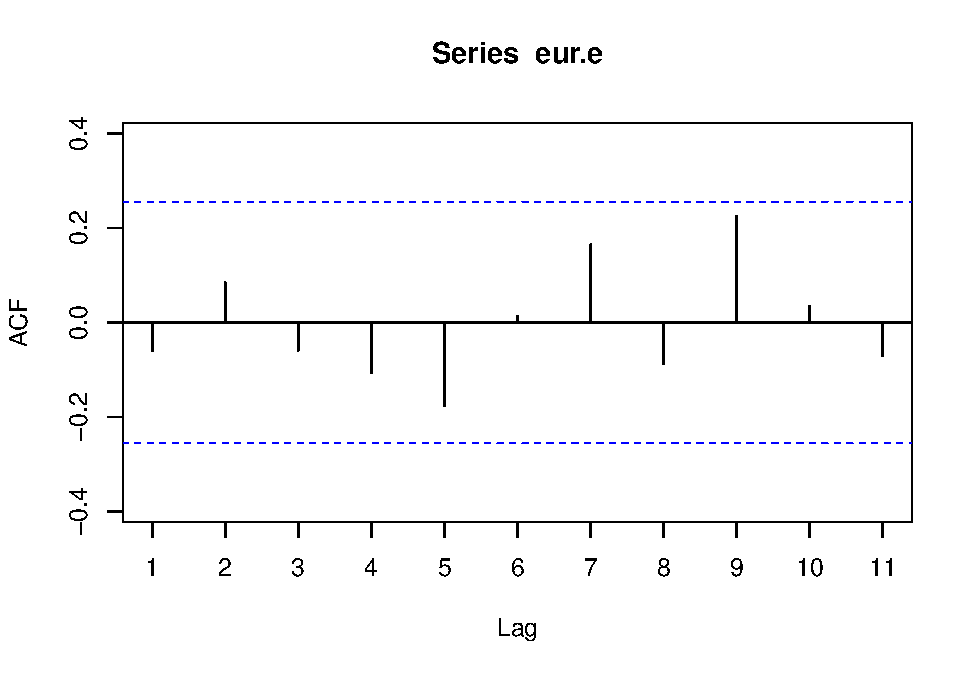
\includegraphics[width=0.5\linewidth]{tsa_files/figure-latex/resid-6}
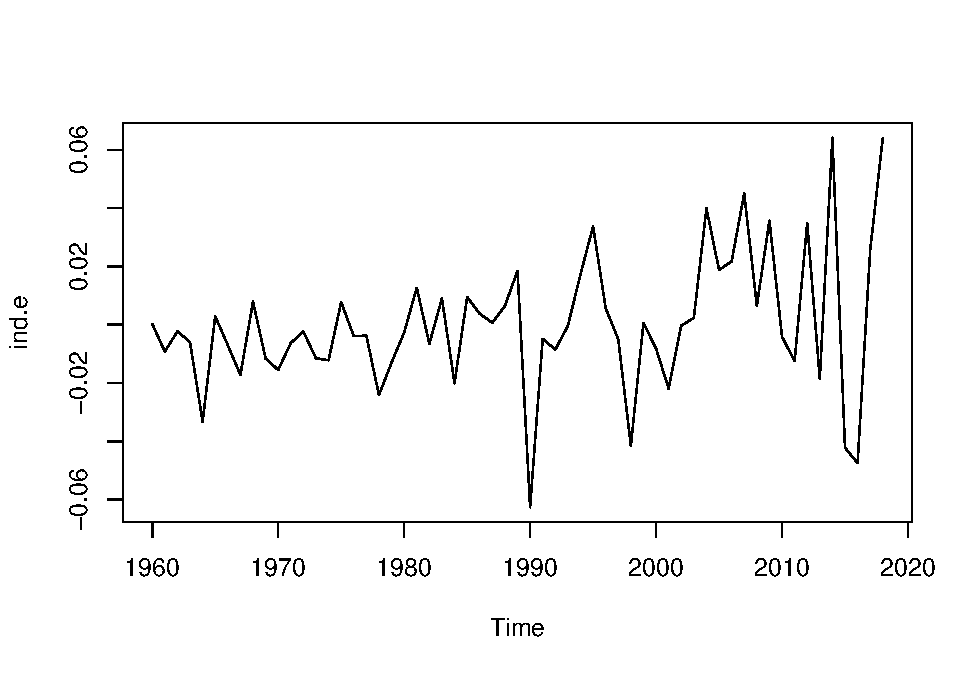
\includegraphics[width=0.5\linewidth]{tsa_files/figure-latex/resid-7}
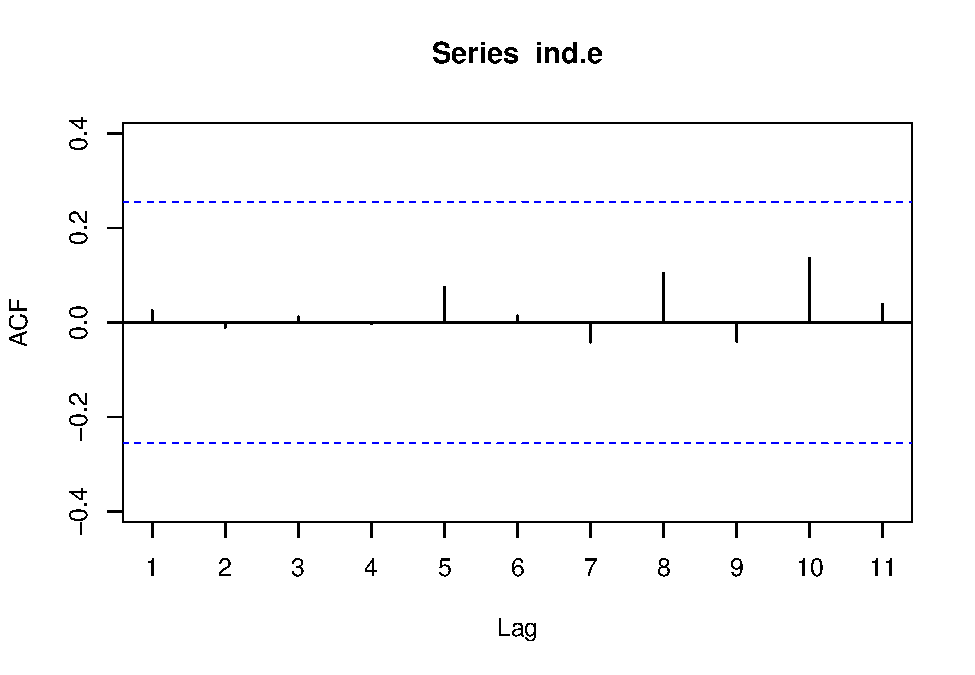
\includegraphics[width=0.5\linewidth]{tsa_files/figure-latex/resid-8}
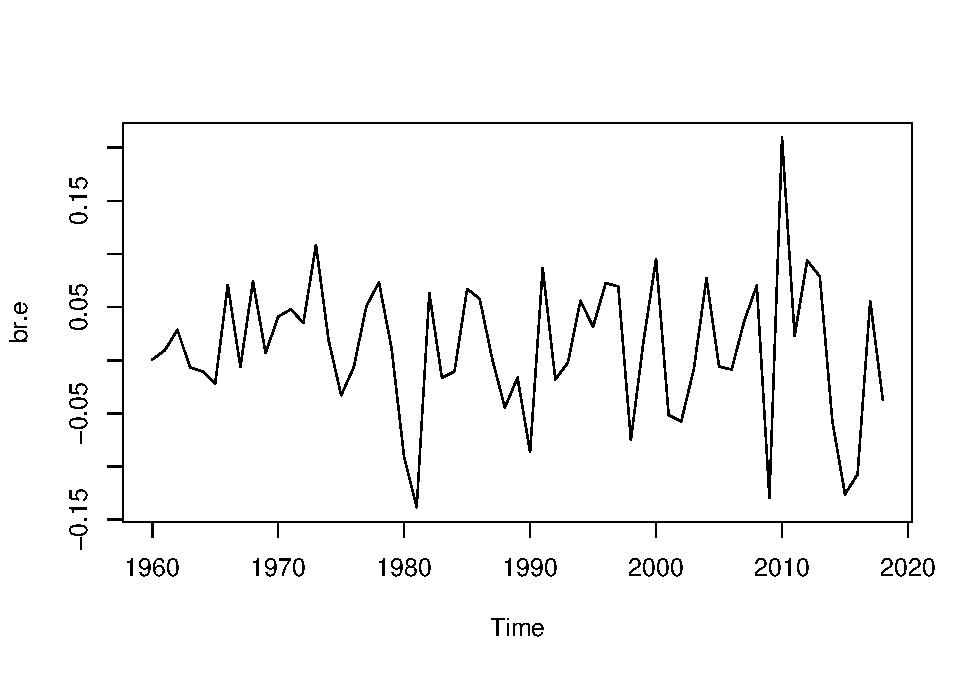
\includegraphics[width=0.5\linewidth]{tsa_files/figure-latex/resid-9}
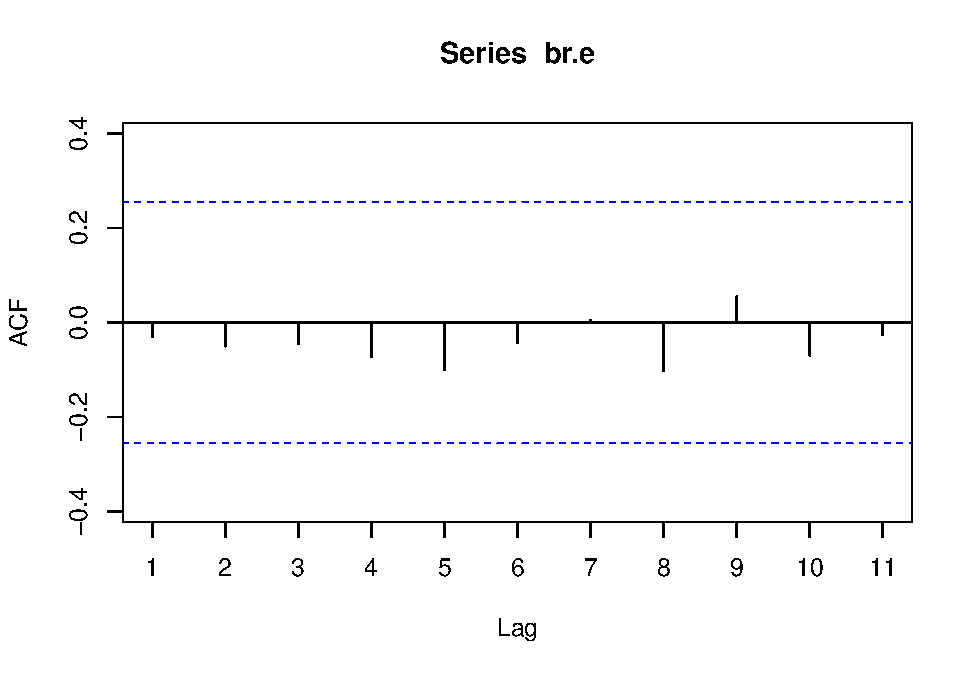
\includegraphics[width=0.5\linewidth]{tsa_files/figure-latex/resid-10}

\hypertarget{forecast}{%
\section{Forecast}\label{forecast}}

Finally, we proceed to forecast carbon dioxide emissions for each
country group until 2030 based on each fitted ARIMA model.

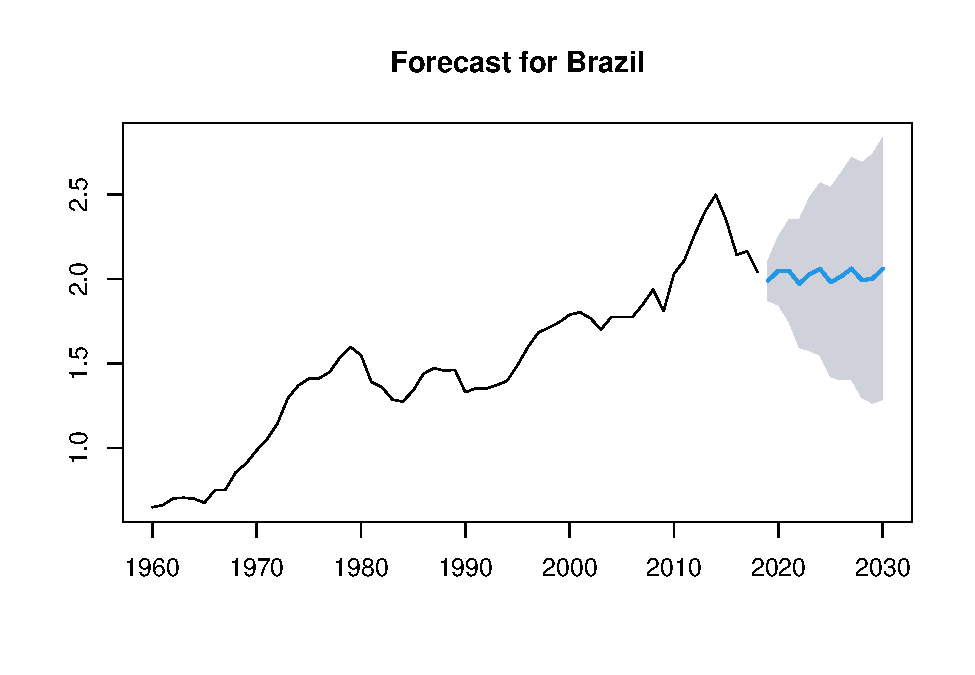
\includegraphics[width=0.5\linewidth]{tsa_files/figure-latex/forecast-1}
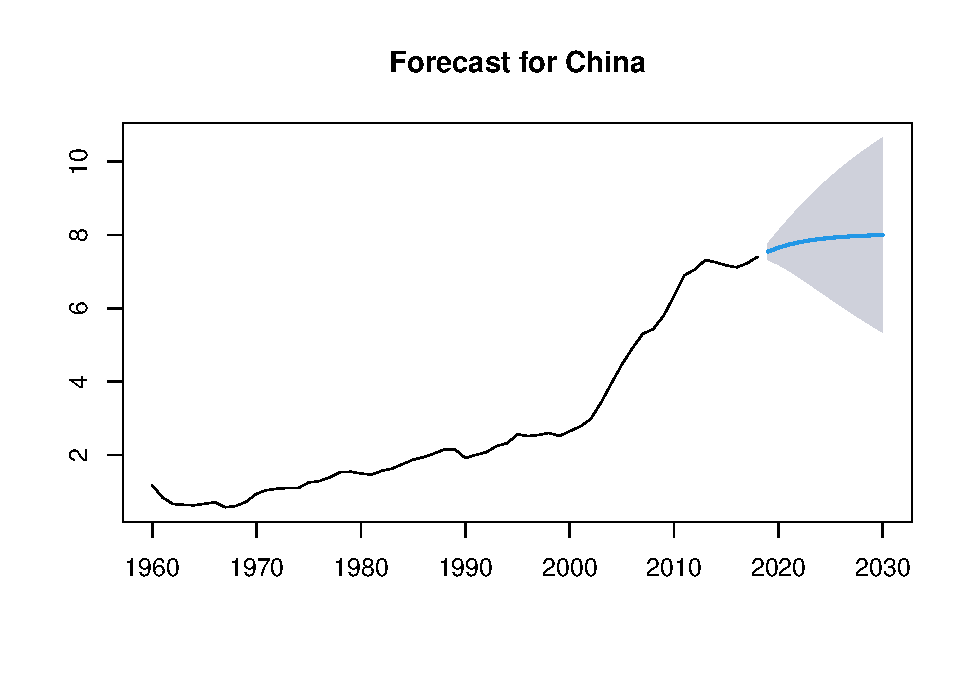
\includegraphics[width=0.5\linewidth]{tsa_files/figure-latex/forecast-2}
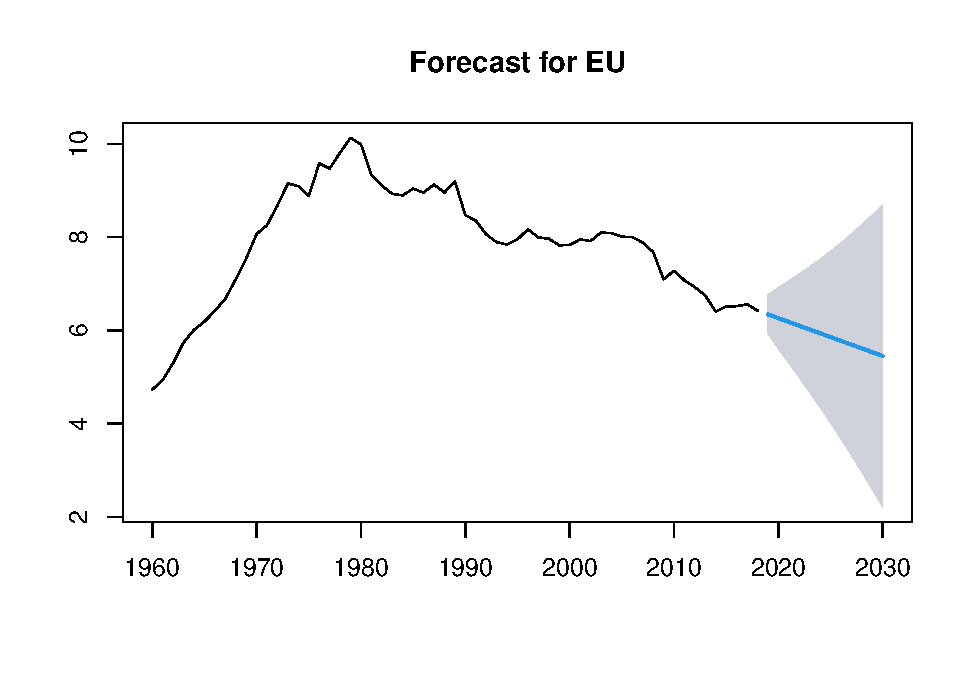
\includegraphics[width=0.5\linewidth]{tsa_files/figure-latex/forecast-3}
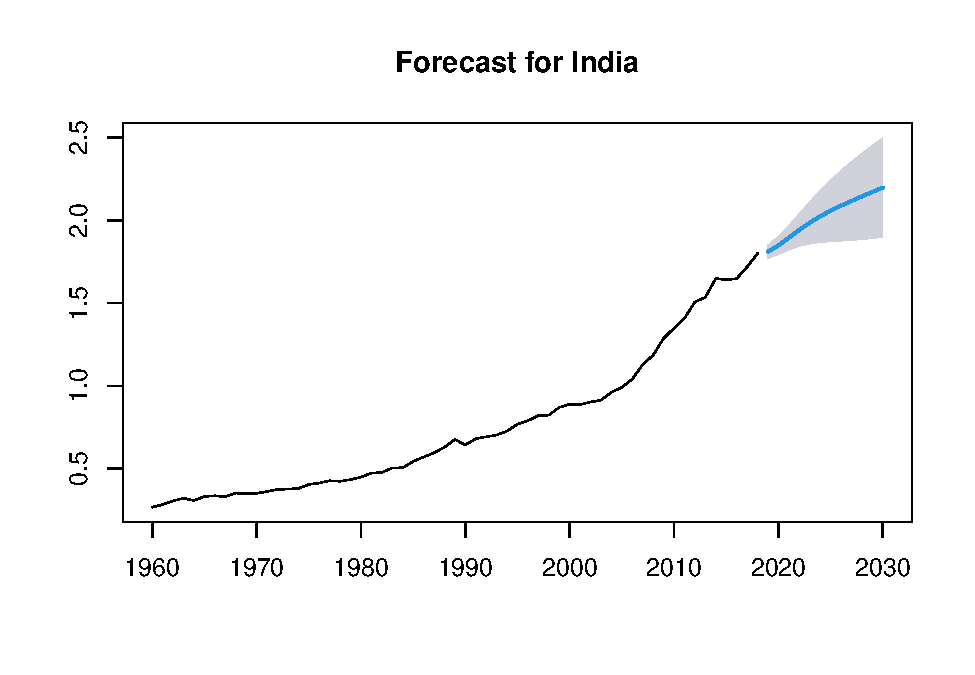
\includegraphics[width=0.5\linewidth]{tsa_files/figure-latex/forecast-4}
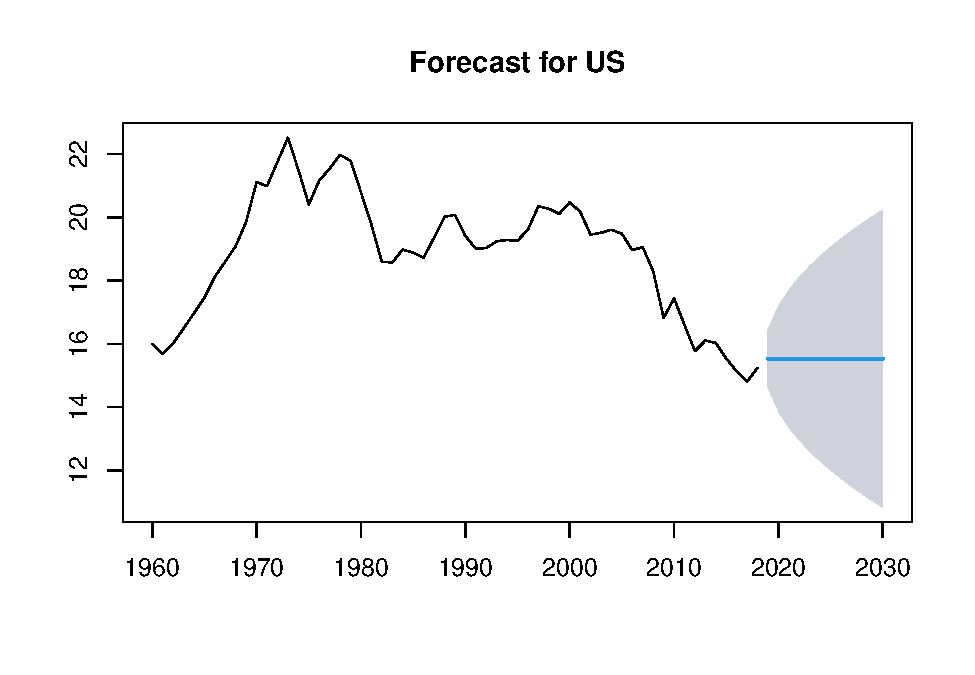
\includegraphics[width=0.5\linewidth]{tsa_files/figure-latex/forecast-5}
The forecast for the different countries show somewhat different
outcomes, in the cases of Brazil and the United States, prediction for
the next 12 periods shows that the emissions will remain stable (within
a 99\% confidence interval). For the cases of China and India, the
forecasted values show some worrying trends, by 2030 both of these
countries will still show rising CO2 emissions, although China's trend
seems to slow down a bit compared to the early 2000's. Luckily, the
forecast for the European Union shows that by 2030, their CO2 emissions
will resemble the ones from the 1960s.

\newpage

\hypertarget{conclusion}{%
\section{Conclusion}\label{conclusion}}

To wrap up this paper we will review the process of the modelling, the
estimation, the diagnostics and the forecasting of the different time
series.

Summing up what has been done, we compared time series from 5 different
countries or country groups, to analyze and model the CO2 emissions
using ARIMA models. Each country shows a different trend, magnitude and
volatily in the data, so different parameters and different models based
on assumptions had to be fitted for each country. We used a variety of a
Grid Search algorithm to navigate through different combinations of
ARIMA (p,d,q) parameters as a way to support our initial stationarity
tests and Auto Correlation Functions. In the end we chose each model
based on the lowest AIC value for each country. Although literature on
CO2 emissions is not particularly scarce, not many authors and
researchers seem to use ARIMA models for this kind of forecasting.
Probably there might exist another advanced techniques that better
forecast CO2 emissions, for example the novel library \emph{prophet} by
Facebook, a collection of forecasting algorithms.

From an environmental point of view, the results and forecast of this
study are negative, though United States and the EU have shown
decreasing trends in their emissions, they are still the two biggest
actors in the world. With China's surprisingly fast emergence in the
global economy, the forecast for them shows the most worrying trend.
China has already surpassed the EU's emissions and though they have
somewhat slowed down the pace, they still show a rising trend. The main
reason for including two other emerging economies like Brazil and India,
was to check if China's disturbing trends also translate into these
countries. Sadly for our environment, the answer is yes, albeit on a
much smaller scale.

Some other factors that could prove to be pivotal in the slow decline of
CO2 emissions in the European Union and USA could be historical events
like the Kyoto Protocol in 1997 and the Paris Agreement in 2015, and
some natural distasters, like the 2011 tsunami in Japan that caused the
explosion in the nuclear factory in Fukushima. This event led to a chain
of events that ended with Germany's (and some other European countries)
abandonment of atomic energy.

\newpage

\hypertarget{appendix}{%
\section{Appendix}\label{appendix}}

For sake of completeness, we include here the differenced plots of the
time series and their respective ACFs.

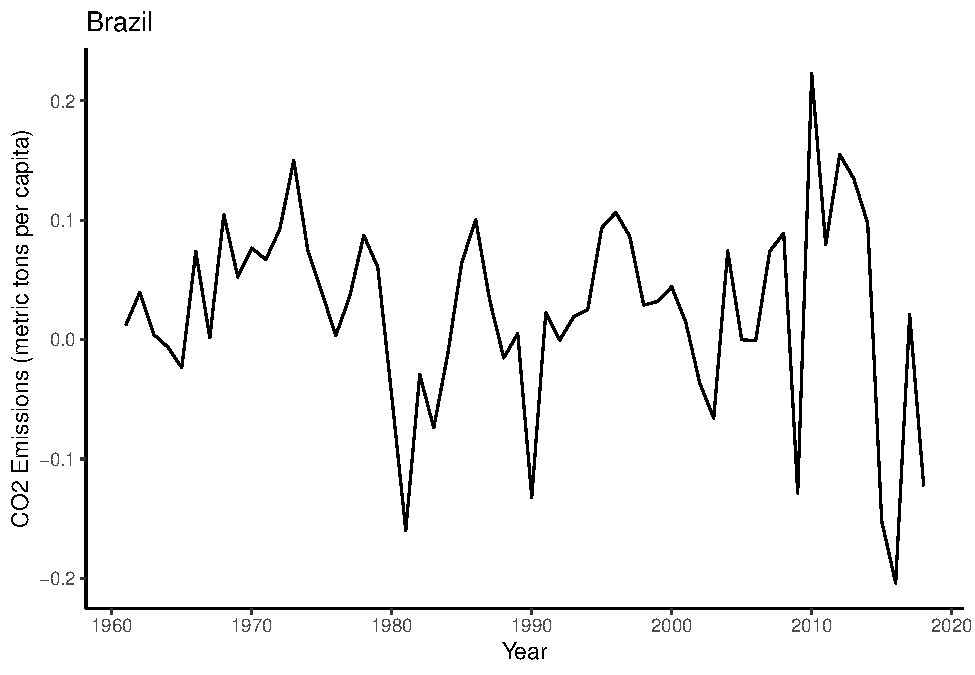
\includegraphics[width=0.5\linewidth]{tsa_files/figure-latex/diffplots-1}
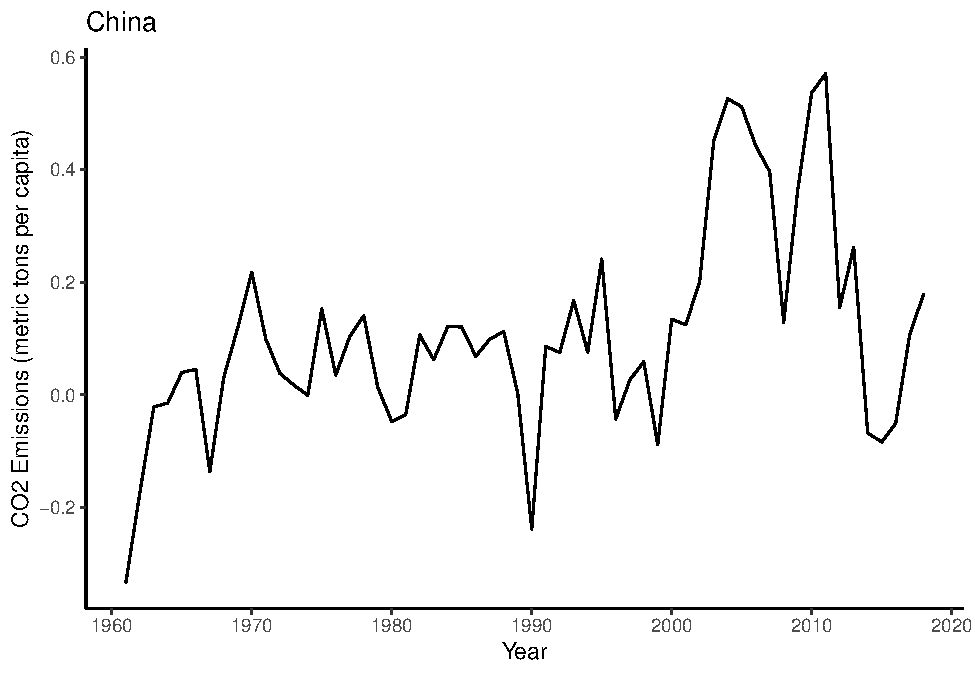
\includegraphics[width=0.5\linewidth]{tsa_files/figure-latex/diffplots-2}
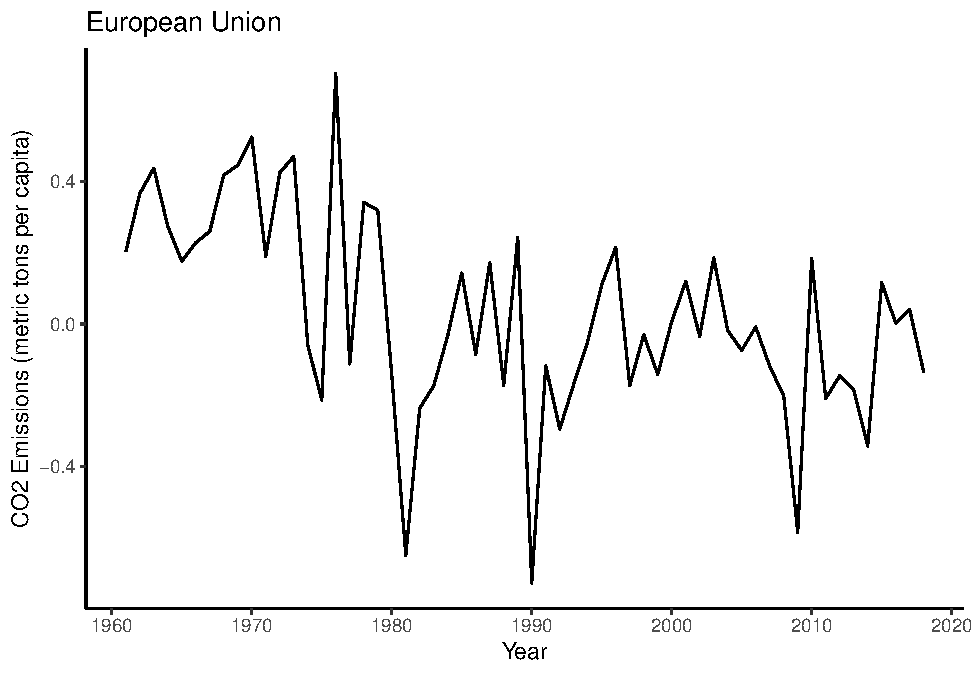
\includegraphics[width=0.5\linewidth]{tsa_files/figure-latex/diffplots-3}
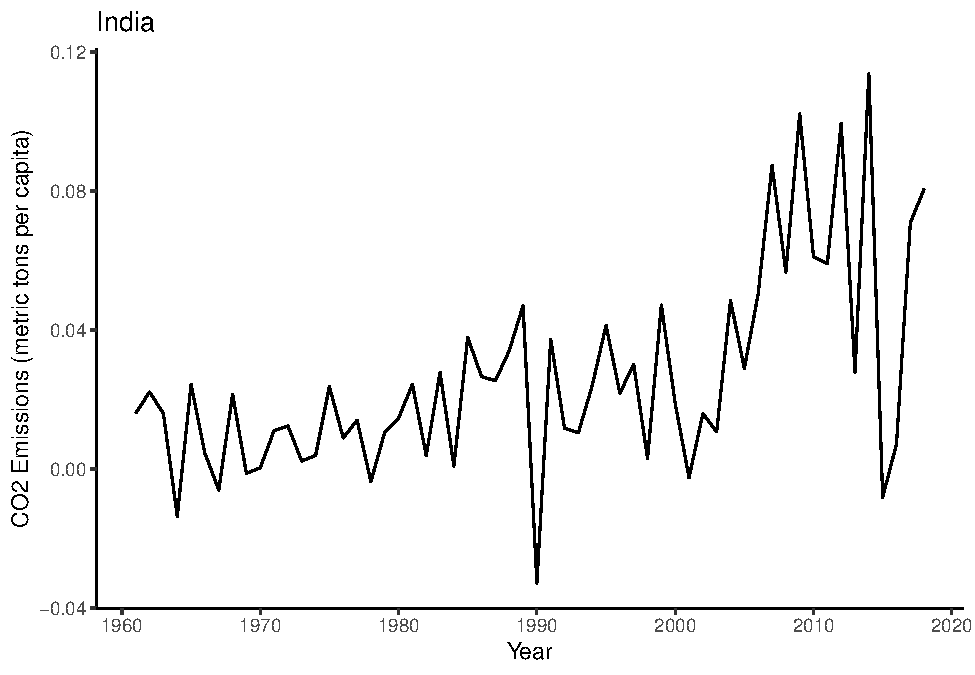
\includegraphics[width=0.5\linewidth]{tsa_files/figure-latex/diffplots-4}
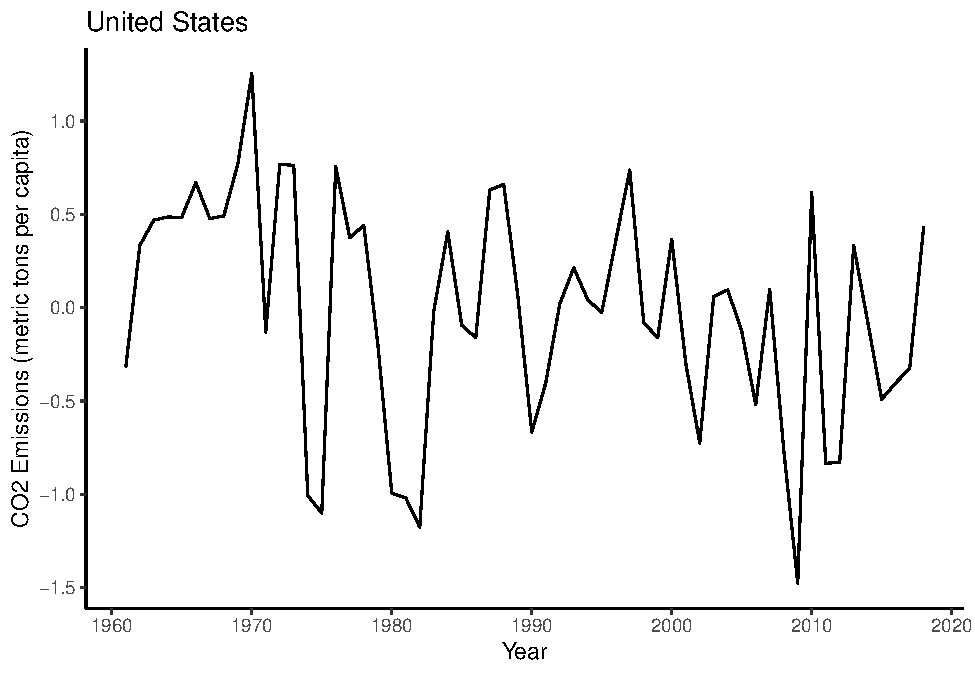
\includegraphics[width=0.5\linewidth]{tsa_files/figure-latex/diffplots-5}

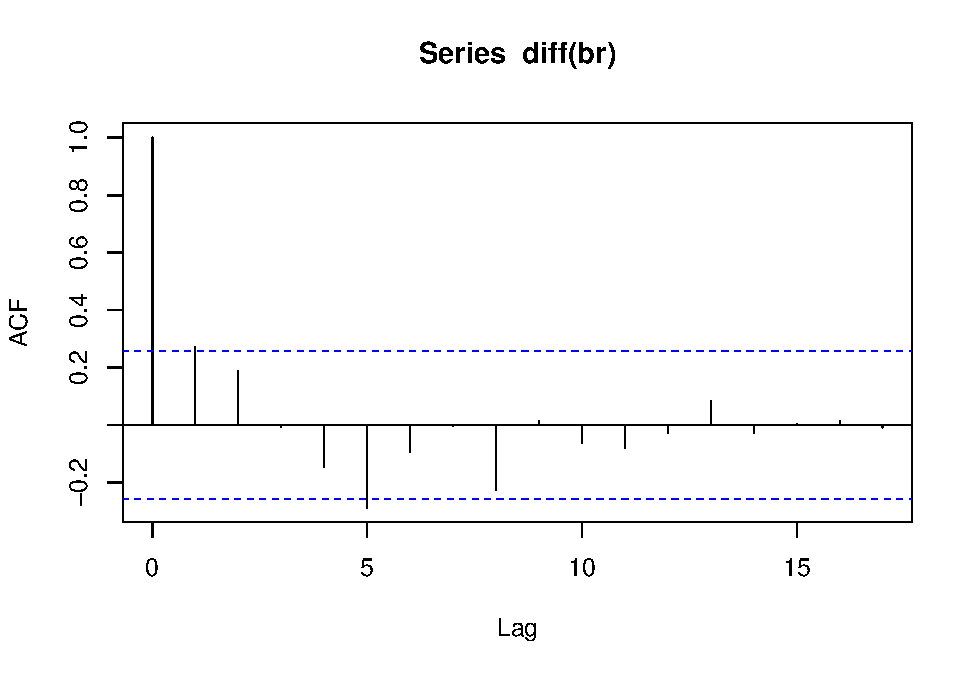
\includegraphics[width=0.5\linewidth]{tsa_files/figure-latex/newacfs-1}
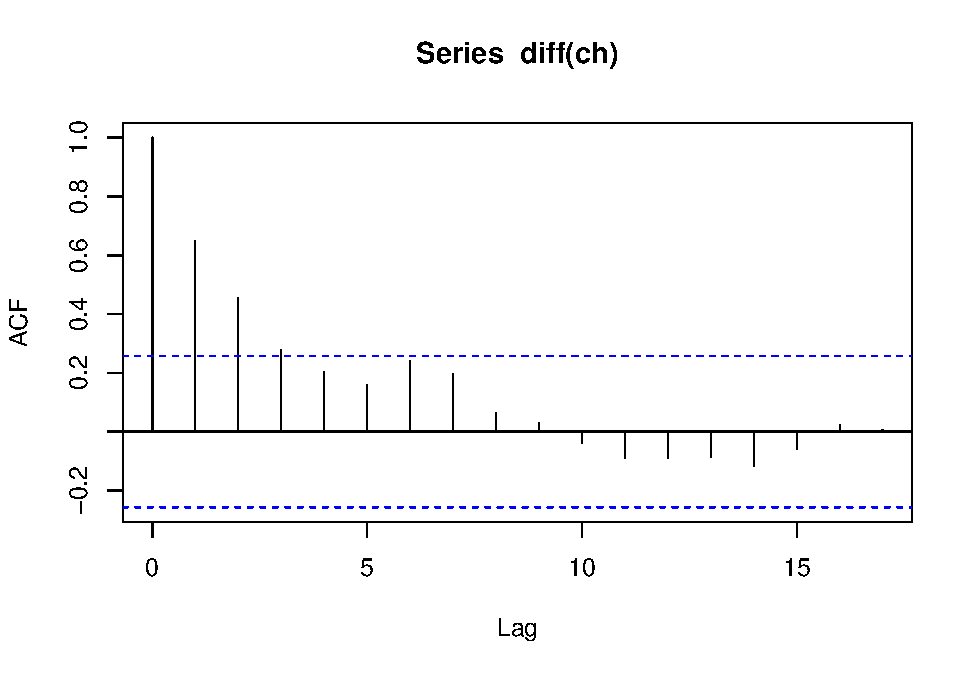
\includegraphics[width=0.5\linewidth]{tsa_files/figure-latex/newacfs-2}
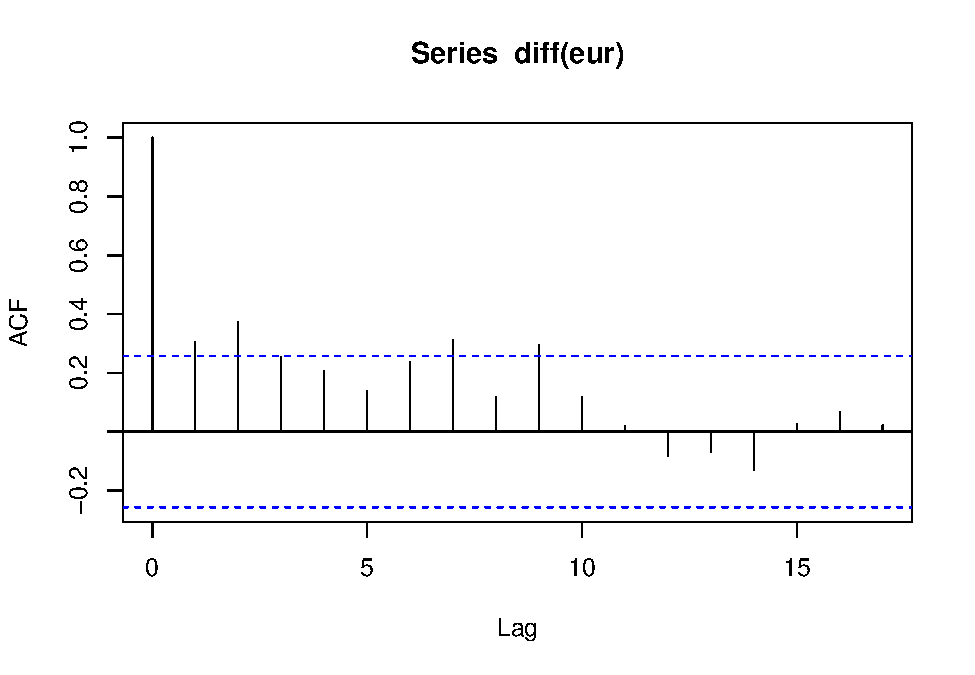
\includegraphics[width=0.5\linewidth]{tsa_files/figure-latex/newacfs-3}
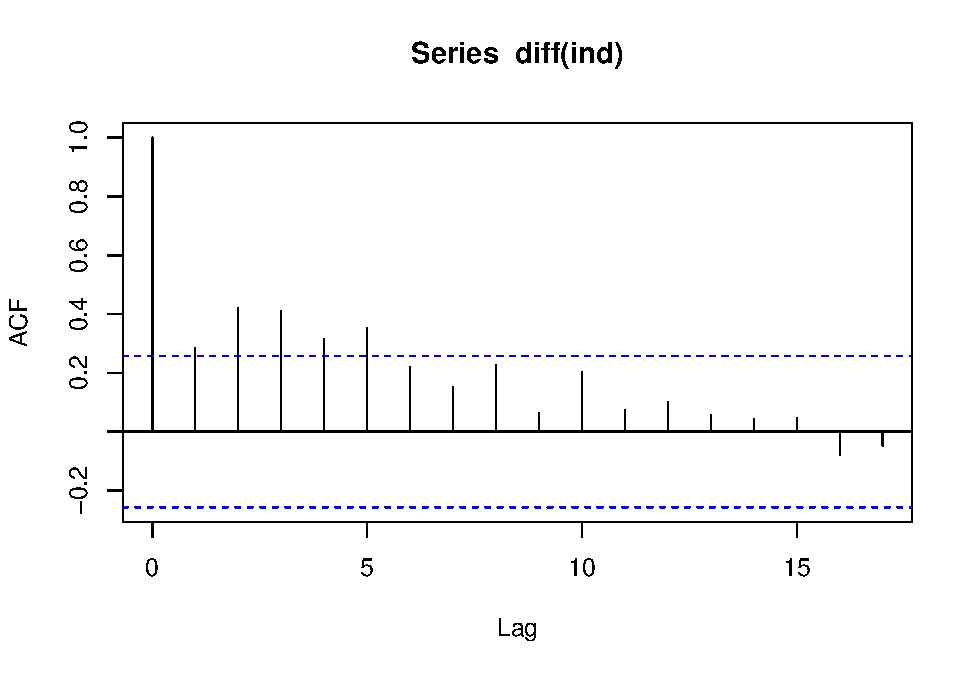
\includegraphics[width=0.5\linewidth]{tsa_files/figure-latex/newacfs-4}
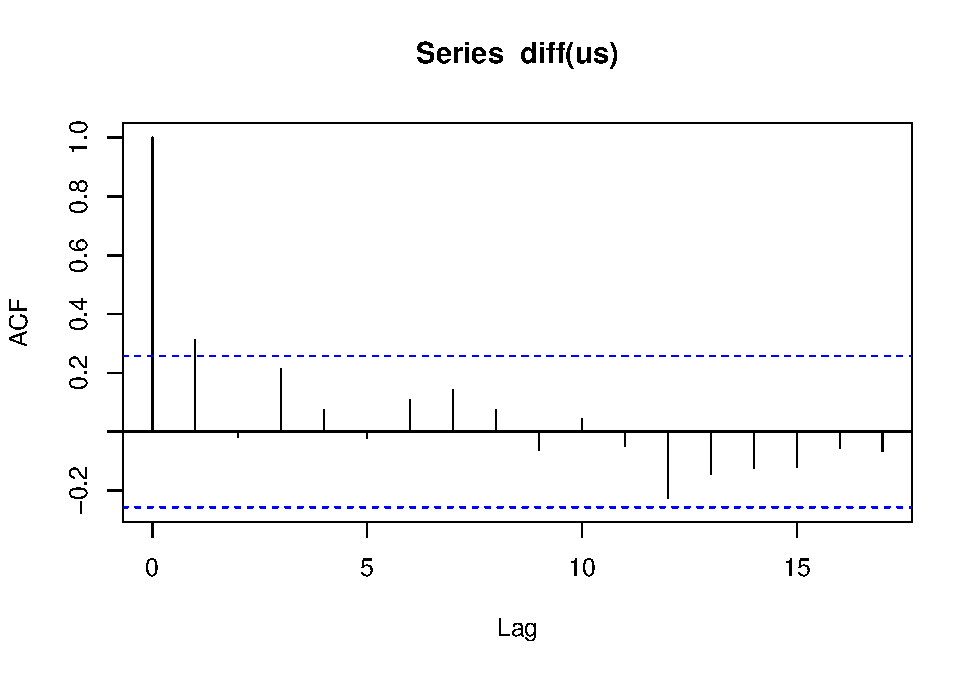
\includegraphics[width=0.5\linewidth]{tsa_files/figure-latex/newacfs-5}

\newpage

  \bibliography{references.bib}

\end{document}
